\documentclass[10pt,a4paper,oneside,abstracton]{scrartcl}
\usepackage[utf8]{inputenc}
\usepackage[english, ngerman]{babel}

\usepackage{gensymb}
% \usepackage[T1]{fontenc}

\usepackage{amsmath}
\usepackage{amsfonts}
\usepackage{amssymb}
\usepackage{graphicx}
\usepackage{lmodern}
	%\usepackage{kpfonts}
\usepackage{fourier}
\usepackage[left=2cm,right=2cm,top=2cm,bottom=2cm]{geometry}
\usepackage{multicol}
\setcounter{secnumdepth}{4} %Nummerierungstiefe bis Paragraph (4. Ebene)
\usepackage{blindtext}
\usepackage[ 		%Einstellungen für Link
   colorlinks,        % Link ohne Umrandungen in zu wählender Farbe 
   linkcolor=black,   % Farbe interner Verweise 
   filecolor=black,   % Farbe externer Verweise 
   citecolor=black    % Farbe von Zitaten 
]{hyperref}



\newenvironment{Figure}
  {\par\medskip\noindent\minipage{\linewidth}}
  {\endminipage\par\medskip}


\pagestyle{empty}		%Seitenzahl wird nich angezeigt

\begin{document}

\section*{Praktische Anwendung einer elektrischen und thermischen Simulation einer Platine zur Ansteuerung eines BLDC-Motors}
\section*{Christian Schmid}
Hochschule Augsburg, Fakultät für Elektrotechnik, Augsburg, Deutschland, Christian.Schmid1@Hs-Augsburg.de 


\begin{abstract} %kann man auch ueber /subsection machen
\noindent %einrücken verhindern
Dies ist ein normaler Text in 10 pt Schriftgröße und 12 pt Zeilenabstand. Dies ist ein normaler Text in 10 pt Schriftgröße und 12 pt Zeilenabstand. Dies ist ein normaler Text in 10 pt Schriftgröße und 12 pt Zeilenabstand. Dies ist ein normaler Text in 10 pt Schriftgröße und 12 pt Zeilenabstand. Dies ist ein normaler Text in 10 pt Schriftgröße und 12 pt Zeilenab-stand. Dies ist ein normaler Text in 10 pt Schriftgröße und 12 pt Zeilenabstand. Dies ist ein normaler Text in 10 pt Schriftgröße und 12 pt Zeilenabstand. Dies ist ein normaler Text in 10 pt Schriftgröße und 12 pt Zeilenabstand. Dies ist ein normaler Text in 10 pt Schriftgröße und 12 pt Zeilenabstand.
\end{abstract}

\renewcommand{\abstractname}{Abstract} %aendert name Zusammenfassung in Abstract

\begin{abstract}
\noindent %einrücken verhindern
Dies ist ein normaler Text in 10 pt Schriftgröße und 12 pt Zeilenabstand. Dies ist ein normaler Text in 10 pt Schrift-größe und 12 pt Zeilenabstand. Dies ist ein normaler Text in 10 pt Schriftgröße und 12 pt Zeilenabstand. Dies ist ein normaler Text in 10 pt Schriftgröße und 12 pt Zeilen-abstand. Dies ist ein normaler Text in 10 pt Schriftgröße und 12 pt Zeilenabstand.
\end{abstract}


\begin{multicols}{2}
\section{Grundlagen}

\subsection{Wärmefluss}
Es gibt 3 Möglichkeiten 
wie sich Wärme ausbreiten kann. Durch Strahlung, Konvektion und Konduktion \cite{Waermefluss}. 
Alle 3 Ausbreitungsmöglichkeiten treten an der Platine auf, siehe Abbildung \ref*{l_Waermefluss}. 

\begin{Figure}
	% \resizebox{0.1\columnwidth}{!} 
	\includegraphics[width=\textwidth]{Bilder/Wärmestrom.png}
	\captionof{figure}{Wärmefluss auf einer Platine, \cite{Waermefluss}}
	\label{l_Waermefluss}
\end{Figure}

\subsection{Thermische Auslegung}
Eletrische Komponenten haben einen Betriebstemperaturbereich. 
Bauteile werden vom Hersteller im Temperaturbereich getestet. 
Aus den Messdaten wird der zu erwartende Lebenszyklus ermittelt.  
Bei überschreiten der Temperatur kann die Lebenszeit der Bauteile rapide abnehmen. 
Besonders gefährdet sind Elektrolyt Kondensatoren. 
Die maximale Temperatur beträgt meist $ 105 \degree C $. \newline 
% Die Lebensdauer der Bauteile halbiert sich jeweils  bei Erhöhung der Betriebstemperatur um jeweils $ 10K $ \cite{Elko}.
Bei Erhöhung der Betriebstemperatur um jeweils $ 10K $ halbiert sich die Lebensdauer der Bauteile \cite{Elko}.
\newline
Um die Verluste und daraus entstehende Abwärme durch Selbstinduktion und elektrische Widerstände  auf der Leiterbahn gering zu halten,
wird die Leiterbahn abhängig von der Anwendung unterschiedlich ausgelegt.
\newline
Eine Versorungsleitung benötigt eine größere Leiterbahnfläche als eine Messleitung, da die Versorungsleitung einen höheren Strom führt. 
Der Strom geht quadratisch in die Leistungsformel ein, siehe Formel \ref*{Leistung_Strom}. 
\begin{equation}
	P_{elektrisch} = P_{Thermisch} =  I^2 \cdot R_{Leiter} 
	\label{Leistung_Strom}
\end{equation}
% \subsection{BLDC-Motor Aussteuerung}
% Der Brushless DC Motor ist eine Synchronmaschine. 
% Eine Synchronmaschine braucht 3 zueinander versetzte Phasen mit Spannungen, die einen sinus darstellen.
% Um die Funktionsweise zu erhalten wird das Stellglied getaktet an und abgeschaltet. 
% Die Schaltfrequenz ist 100 - 10.000 so groß wie die gewollte Winkelgeschwindigkeit. 
% Die Schaltfrequenz ist zu groß für das System. (vgl. Abbildung \ref*{Aussteuerung})
% \newline
% Es stellt sich eine mittlere Spannung ein, die sich über der Zeit nur langsam verändert.
% Das System folgt der dem Sollsignal.

% \begin{Figure}
% 	% \resizebox{0.1\columnwidth}{!} 
% 	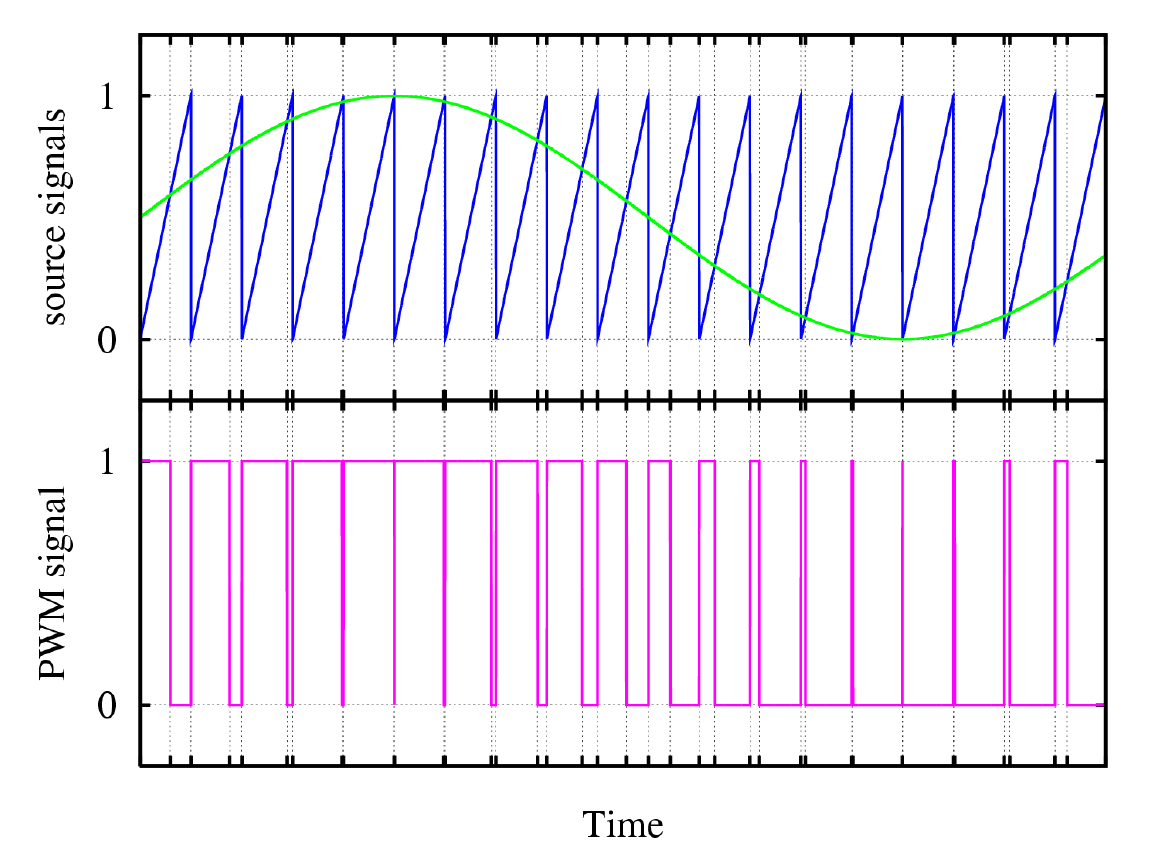
\includegraphics[width=\textwidth]{Bilder/BLDC_Aussteuerung.png}
% 	\captionof{figure}{Aussteuerung einer Phase, \cite{Vorlesung Aussteuerung}}
% 	\label{Aussteuerung}
% \end{Figure}

% \noindent
% Die Schematische Funktionsweise eines Brushless DC Motors sieht wie folgt aus. 
% Mittels 3 Halbbrücken werden die drei Phasen des Motors getrennt angesteuert und der Motor gesteuert, 
% beziehungsweise geregelt(vgl. Abbildung \ref*{Motor_Schematic}). 
% Die Geschwindigkeit wird vorgegeben, indem die Winkelgeschwindigkeit $ \omega $ eingestellt wird. 
%  $ \omega = 2\pi \cdot n = \frac{d\varphi}{dt} $   
%  \newline
% Die Spulenspannung wird durch $ u(t) = U \cdot sin(\omega \cdot t + \varphi_U) $ eingestellt. 
% \begin{Figure}
% 	% \resizebox{0.1\columnwidth}{!} 
% 	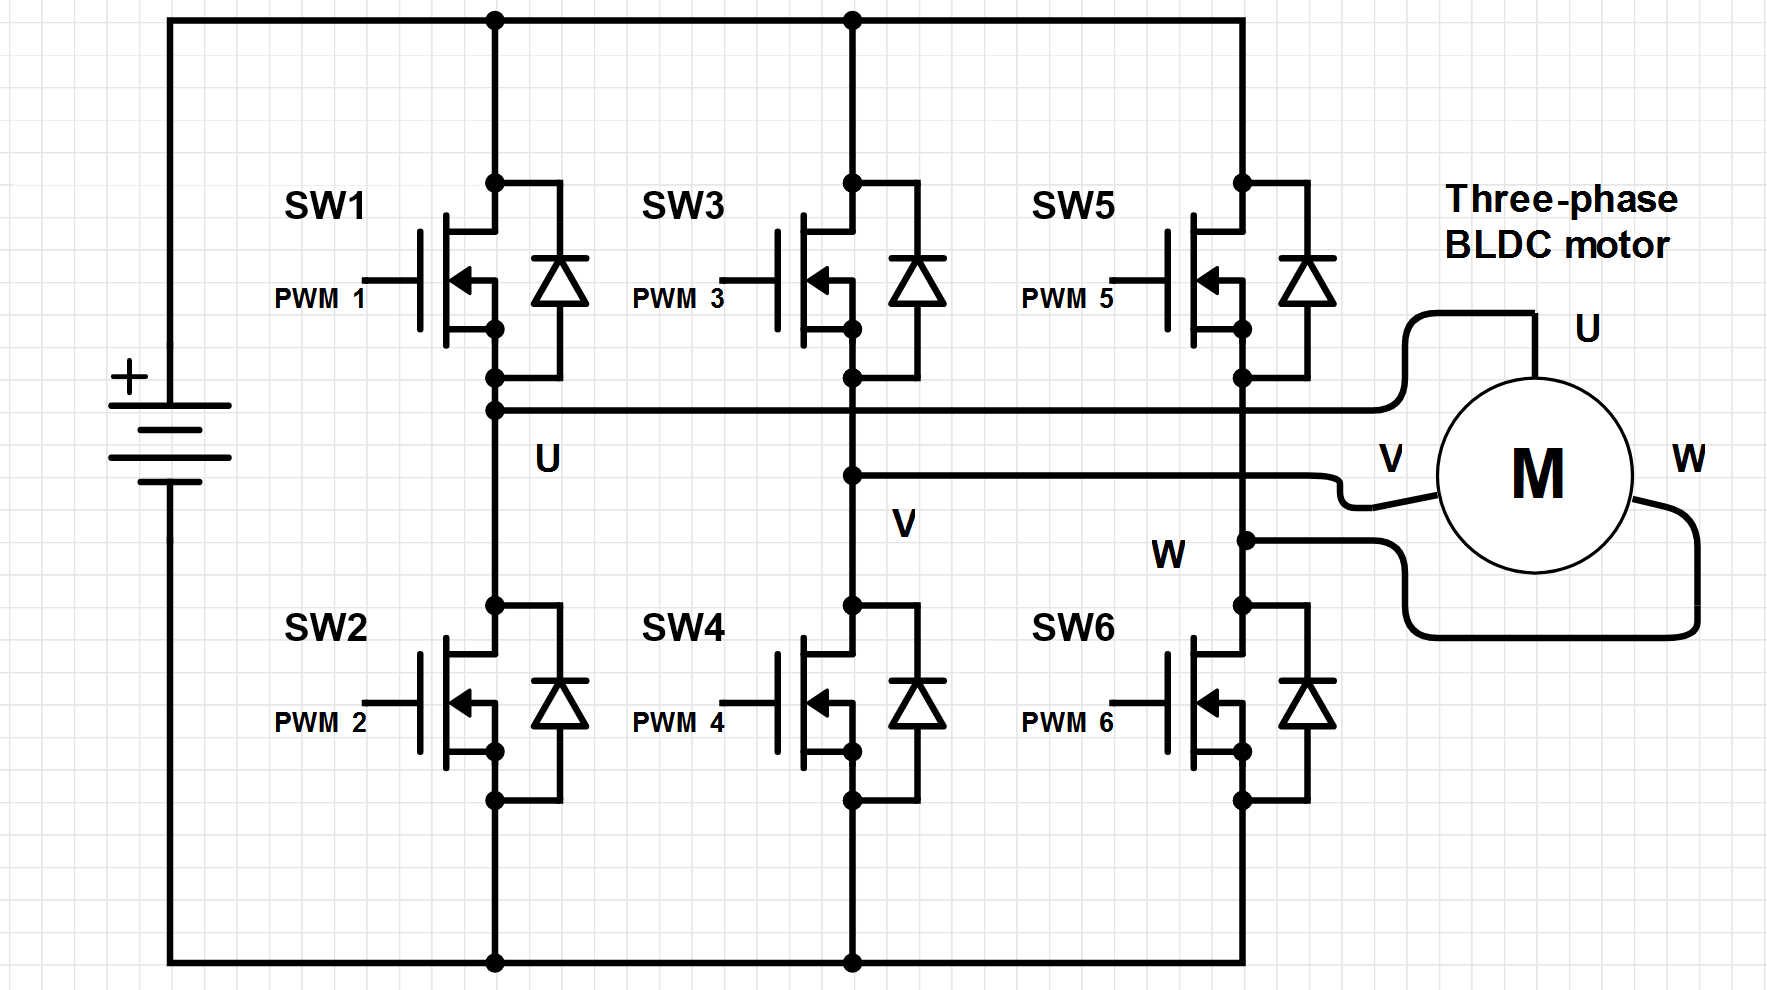
\includegraphics[width=\textwidth]{Bilder/BLDC_Schematic.png}
% 	\captionof{figure}{Schematische Funktionsweise eines BLDC Motors \cite{Motor_Ansteuerung}}
% 	\label{Motor_Schematic}
% \end{Figure}

% \subsubsection{Folgerung}
% Da sich der eingestellte Strom sehr schnell verändert und das Thermische System langsamer ist als die Motoransteuerung, 
% kann davon ausgegangen werden, dass in den Leitungen ein konstanter Strom fließt. 
% Es wird angenommen dass bei maximalem Drehmoment ein Strangstrom von bis zu $I_{Strang} = 5 A $  fließt. 

\section{Thermisches Design}
Abhängig von dem eingestellten Strom gibt es in der Industrie Vorgaben, 
wie breit Leiterbahnen sein sollen. \newline

\subsection{Aufbau einer Platine}
Der Aufbau einer 2 lagigen Platine ist in Abbildung \ref*{pcb_im} dargestellt. 
\newline
Die mittlere Schicht der Platine besteht aus FR4, einem $ 1,5mm $ breiten Dielektrikum \cite{PCB_Querschnitt}. 
Die Leiterbahnenhöhe auf Ober- und Unterseite betragen $ 35 \mu m$ \cite{aisler}.
\begin{Figure}
	% \resizebox{0.1\columnwidth}{!} 
	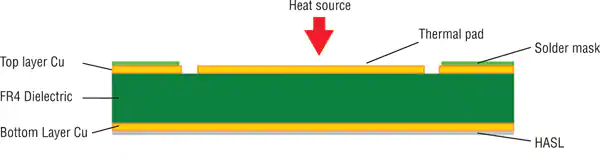
\includegraphics[width=\textwidth]{Bilder/PCB_Querschnitt.png}
	\captionof{figure}{Querschnitt einer  Platine \cite{PCB_Querschnitt}}
	\label{pcb_im}
\end{Figure}

\noindent
Mittels Vias kann die Wärmeenergie einfacher durch die Platine fließen. 
Dieser Fall wird nicht untersucht.
% Die Wärme fließt durch das Dielektrikum und auch über die Luft. 

\noindent



\subsection{Überprüfung des Vorgabewerts}
Die Arbeit widmet sich der Bestimmung des Thermischen Widerstands und der 
Platinenerwärmung durch den eingestellten Strom. 
\newline
Für einen Strom von $I_{Strang} = 5 A $ und einer maximalen Erwärmung von $10 K$ ergibt sich nach dem Industriestandard eine
Leiterbahnbreite von $b = 4 mm $ \cite{ipc}. \newline
Für die Arbeit wird ein Strom von $I_{Strang} = 5 A $ und eine Leiterbahnbreite von $b = 4 mm $ untersucht.
Die Platine hat die Maße $15mm x 15mm$
Die Abmaße der zu simulierende Platine sind in Abbildung \ref*{geometry} ersichtlich.


\begin{Figure}
	% \resizebox{0.1\columnwidth}{!} 
	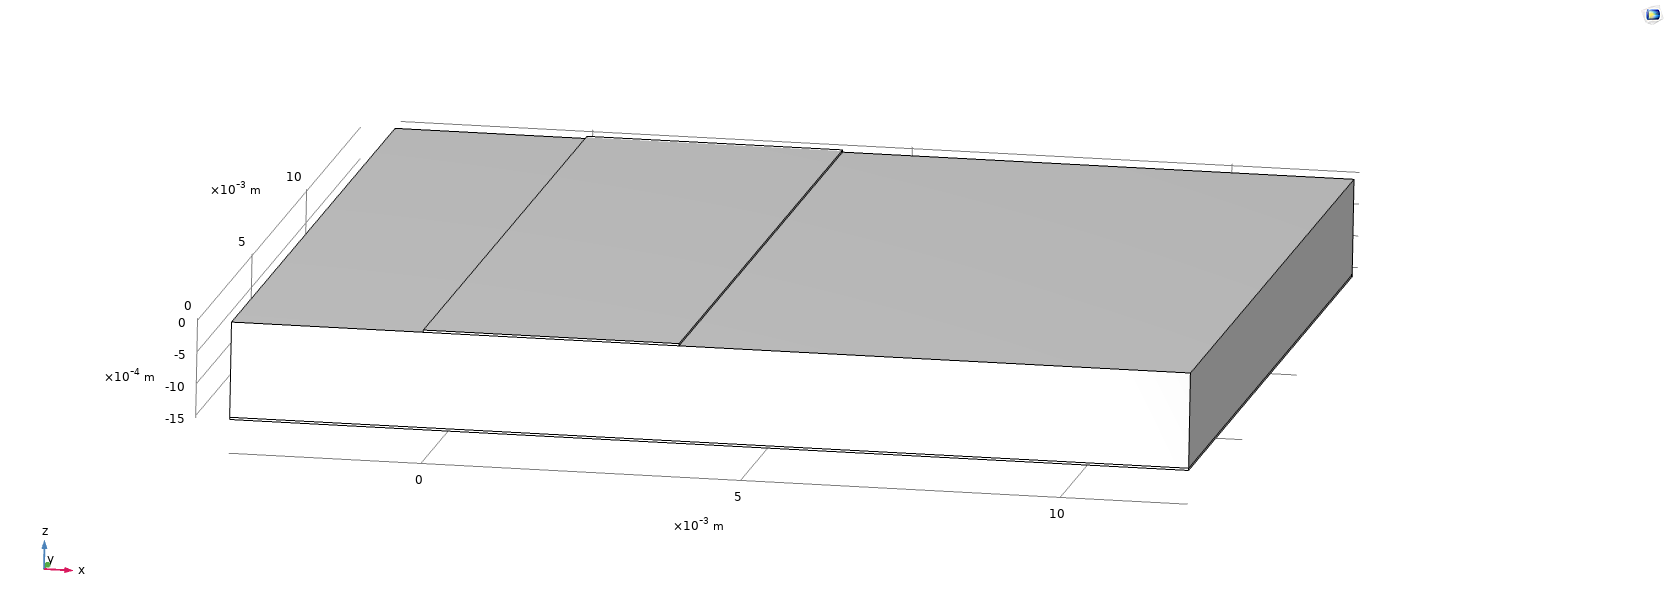
\includegraphics[width=\textwidth]{Bilder/Geometrie.png}
	\captionof{figure}{Geometrie der verwendeten Platine}
	\label{geometry}
\end{Figure}

\subsection{Wärmestrom}
Der Wärmestrom wird durch den elektrischen Strom der Leiterbahn und den Widerstand des Leiters bestimmt. 
\newline
Die elektrische Leitfähigkeit von Kupfer betragt $ \rho_{Cu} = \frac{58.1\cdot 10^6}{Sm^{-1}} $.
\newline
Die zu simmulierende Leiterbahnlänge betragt $l = 15 mm$.
\newline
Die Querschnittsfläche der Leiterbahn betragt: 
\begin{equation}
	A = b \cdot h = 4 mm \cdot 35 \mu m = 140 m^{-9}
\end{equation}
Der Widerstand der Leiterbahn betragt: 
\begin{equation}
	R_{Leiter} = \frac{1}{\rho} \cdot \frac{l}{A} = 1,84 \cdot 10^{-3} \Omega
\end{equation}
\noindent
Der elektrische Schaltplan ist in Abbldung \ref*{Schaltplan} ersichtlich.  \newline
Es stellt sich eine Spannung über dem Widerstand ein, vgl. Formel \ref*{Spannung}. 
\begin{equation}
	U_{Verlust} =  I_{Strang} \cdot R_{Leiter} 
	\label{Spannung}
\end{equation}
\noindent
Die elektrische Verlustleistung wird mit Formel \ref*{Verlustleistung} berechnet: 
\begin{equation}
	P_{elektrisch} = P_{Thermisch} =  I^2 \cdot R_{Leiter} 
	\label{Verlustleistung}
\end{equation}
Es wird
$ P_{Thermisch} = (5A)^2 \cdot 1,84 \cdot 10^{-3} \Omega = 46 \cdot 10^{-3} W $ \newline
in das System eingeprägt.
Die Erwärmung wird mit Formel \ref*{Erwaermung} berechnet.
\begin{equation}
	\Delta T = P_{Thermisch} \cdot \Theta_{Junction, Ambient}
	\label{Erwaermung}
\end{equation}





\section{Händische Rechnung}
% Eine erste Näherung um die Erwärmung zu bestimmen lautet: 

% \begin{equation}
% 	\Theta_{Junction, Case} = 10 \frac{K }{W} 
% \end{equation} 
% Die Erwärmung beträgt anhand dieser Regel, vgl. Formel \ref*{Erwaermung}: 

% \noindent
% $\Delta T = 46 \cdot 10^{-3} W \cdot 10 \frac{K }{W} = 0.46 K  $ 
% Die Platine erwärmt sich nach der Formel um $ 0,46 K$.
% \newline
% Die Formel ist sehr allgemein. Es werden keine spezifischen Daten der Platine benötigt, ausschließlich die Wärmeleistung. 

% \subsection{Herleitung der Daumenregel}
\noindent
% Die Berechnung der Erwärmung erfolgt mit dem thermischen Widerständen $\Theta$. Es wird ein Ersatzschaltbild entworfen. 
Der thermische Widerstand $\Theta_{Junction, Case}$  wird mittels Formel \ref*{formel} berechnet . 
\begin{equation}
	\Theta_{Junction, Ambient} = \frac{\frac{1}{h}}{A}
	\label{formel}
\end{equation}
Der Wärme-Transfer-Koeffizient zwischen Platine und Umgebung $\Theta_{Junction, Ambient}$ wird mit $ h = 10 \frac{W}{m^2K}$ angenommen.\newline
Die Oberseite und Unterseite der Platine betragen: \newline
$A = 2\cdot 15mm \cdot 15mm$. 

\begin{equation}
	\Theta_{Junction, Ambient} = \frac{\frac{1}{10 \frac{W}{m^2K}}}{ 2\cdot 15mm \cdot 15mm} = 222 \frac{K}{W}
	\label{formel}
\end{equation}
Die Platine erwärmt sich nach der Formel um \newline
$\Delta T = 46 \cdot 10^{-3} W \cdot 222 \frac{K }{W} = 10.2 K  $.

\section{Elektrischer Schaltplan für den Wärmestrom }
Um den Wert genauer zu bestimmen wird Ersatzschaltbild erstellt um Thermische Verläufe abzubilden.
Es werden die thermischen Widerstände berechnet. 
Das Ersatzschaltbild wird ohne thermische Kapazitäten dargestellt, da uns der statische Zustand interessiert, nicht der transiente.
Um das System noch von Hand zu simmulieren, wird angenommen, dass der Wärmestrom nur nach oben und nach unten fließt. 
Der thermische Widerstand wird durch Formel \ref*{thermischerWiderstand} berechnet. 
\begin{equation}
	\Theta =  \frac{h}{A \cdot \lambda}
	\label{thermischerWiderstand}
\end{equation}
\noindent
\begin{Figure}
	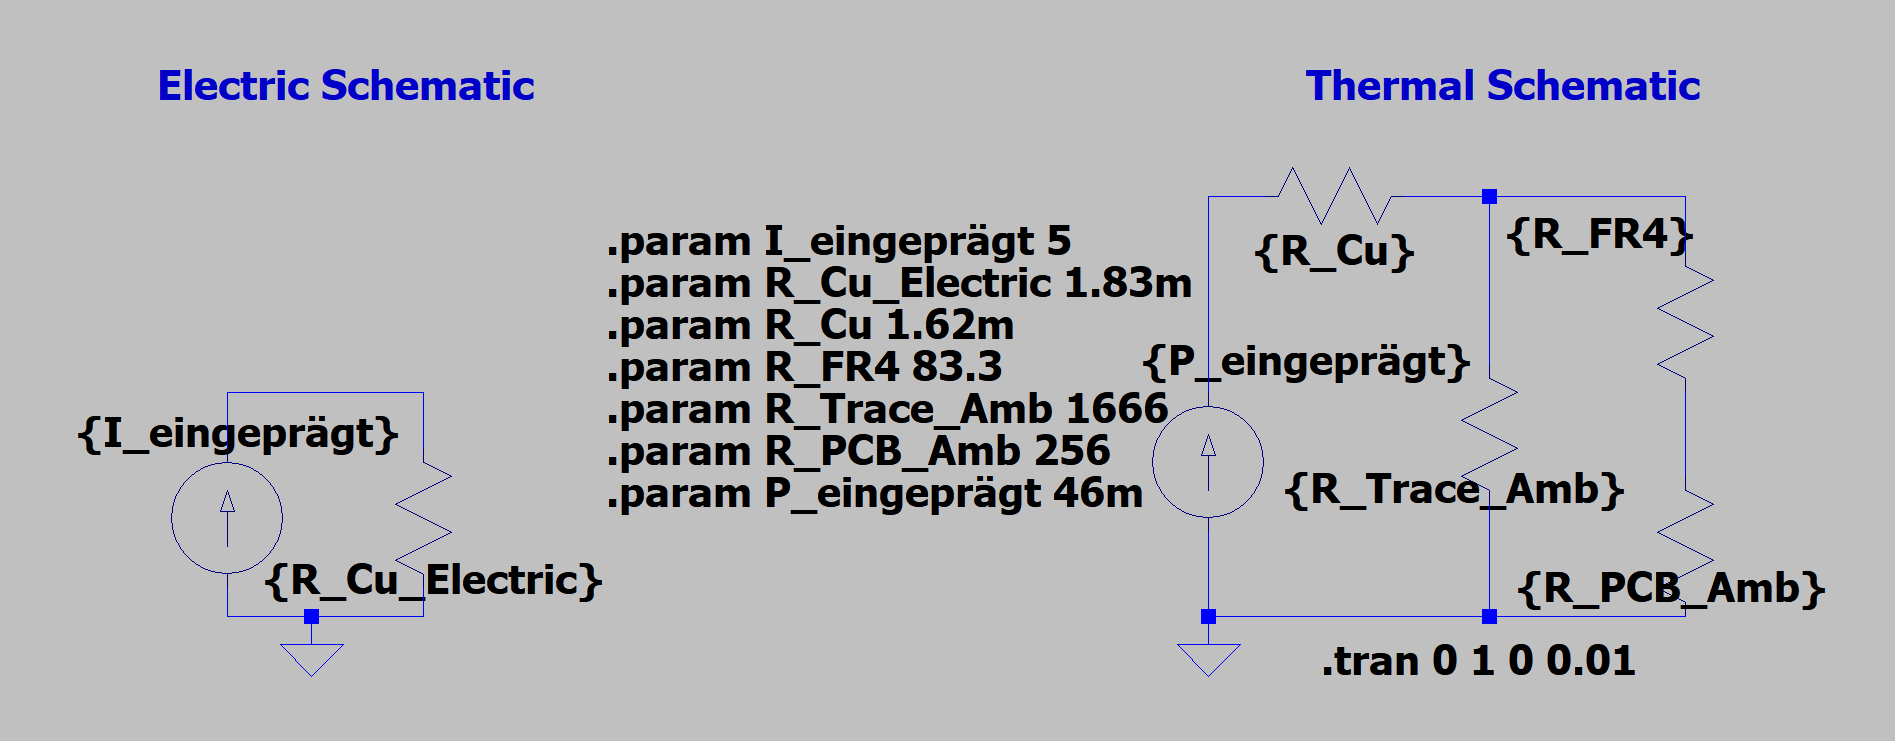
\includegraphics[width=\textwidth]{Bilder/Schaltplan.png}
	\captionof{figure}{Ersatzschaltbild den elektrischen Stromkreis (links) und für die statische Temperatur (rechts)}
	\label{Schaltplan}
\end{Figure}
\noindent
Die Leistung in Abbildung \ref{Schaltplan} stellt den Strom dar. Die Spannung ist die Temperaturerhöhung zur Referenztemperatur. 
Die Platine erwärmt sich um knapp $\Delta T = 13K$
Die thermische Leitfähigkeit von Kupfer beträgt:  \newline 
$\lambda_{Cu} = 360 \frac{W}{m K}$  \cite{Waermefluss} \newline
Für den spezifischen Fall betragt der thermische Widerstand von der Leiterbahn:  \newline
$\Theta_{Leiterbahn} = \frac{35 \mu m}{4mm \cdot 15mm \cdot 360 \frac{W}{m\cdot K}} = 1,62\cdot 10^{-3} \frac{K}{W}$
\newline 
Die thermische Leitfähigkeit von FR4 beträgt: 
\newline
 $\lambda_{FR4} = 0,3 \frac{W}{m K}$ \cite{Waermefluss} \newline
Für den spezifischen Fall betragt der thermische Widerstand von dem Dielektrikum: \newline
$\Theta_{FR4} = \frac{1,5 mm}{mm \cdot 15mm \cdot 0,3 \frac{W}{m\cdot K}} = 1,62\cdot 10^{-3} \frac{K}{W}$
Der thermische Widerstand zwischen Leiterbahn und Ambient beträgt: 
$\Theta_{Leiterbahn, Ambient} = \frac{\frac{1}{10 \frac{W}{m^2K}}}{ 2\cdot 15mm \cdot 15mm - 4mm \cdot 15mm} = 256 \frac{K}{W} $
Der thermische Widerstand zwischen Platine ohne Leiterbahn und Ambient beträgt: 
$\Theta_{PCB, Ambient} = \frac{\frac{1}{10 \frac{W}{m^2K}}}{  4mm \cdot 15mm} = 1666 \frac{K}{W} $

\section{Simulation}
Ein Strom wird an einem Ende eingeprägt. Die Masse ist am anderen Ende. 
Die Geometrie ist in Abbildung \ref*{geometry} ersichtlich. Die Vernetzung ist in Abbildung \ref*{net}.
Da die breiten sich deutlich voneinander unterscheiden, konnte nur eine endliche Fläche für die Platine betrachtet werden.
Bei zu groß gewählter Fläche tritt ein Fehler auf: Einige Kanten sind zu kurz, einige Flächen sind zu schmaal beziehungsweise. 
Auch konnte nur eine endliche Fläche untersucht werden, da sont die Rechenvorgänge zu lange zum simmulieren dauern. 


\begin{Figure}
	% \resizebox{0.1\columnwidth}{!} 
	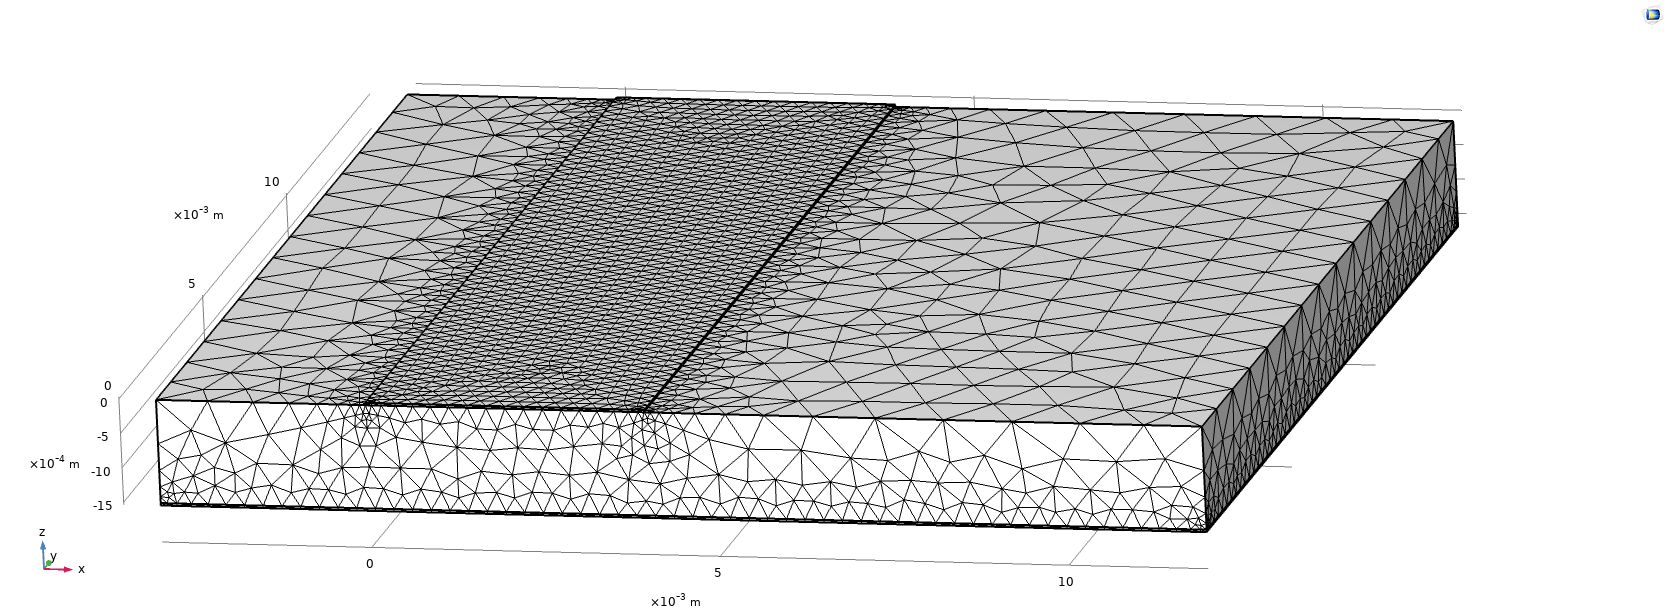
\includegraphics[width=\textwidth]{Bilder/net.png}
	\captionof{figure}{Vernetzung des Models}
	\label{net}
\end{Figure}


\begin{Figure}
	% \resizebox{0.1\columnwidth}{!} 
	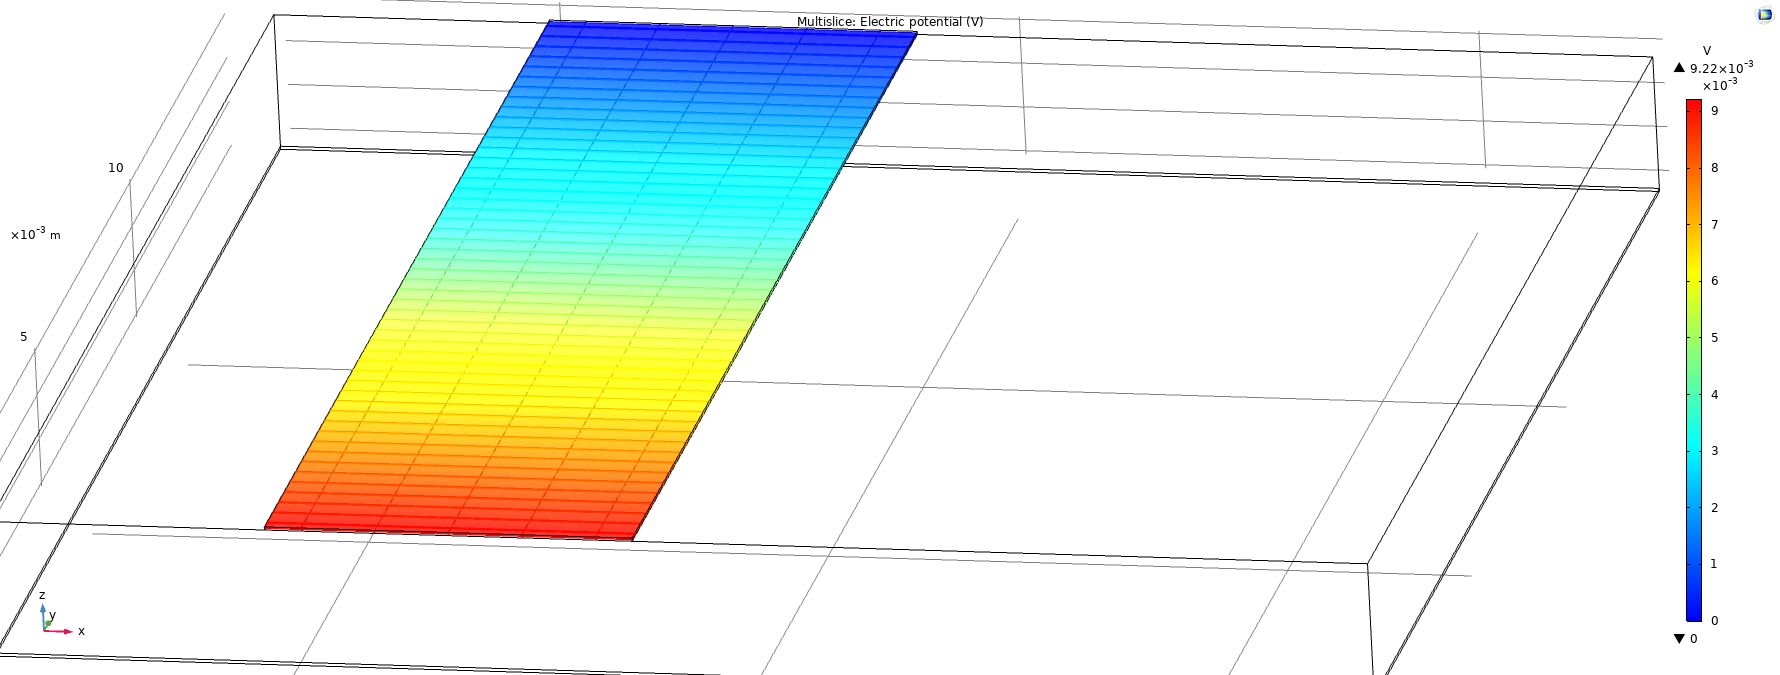
\includegraphics[width=\textwidth]{Bilder/voltage.png}
	\captionof{figure}{Spannungsabfall über der Leiterbahn}
	\label{voltage}
\end{Figure}

\begin{Figure}
	% \resizebox{0.1\columnwidth}{!} 
	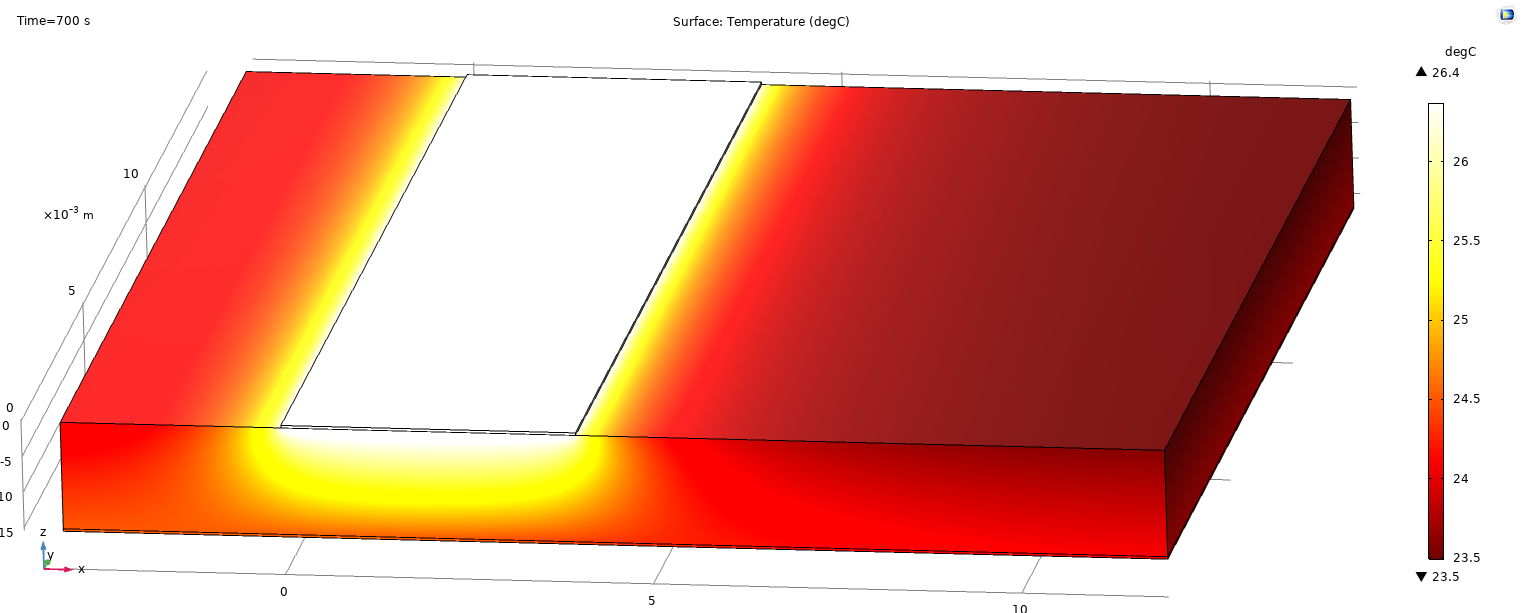
\includegraphics[width=\textwidth]{Bilder/Thermal_static.png}
	\captionof{figure}{Thermische Endzustände}
	\label{voltage}
\end{Figure}

\begin{Figure}
	% \resizebox{0.1\columnwidth}{!} 
	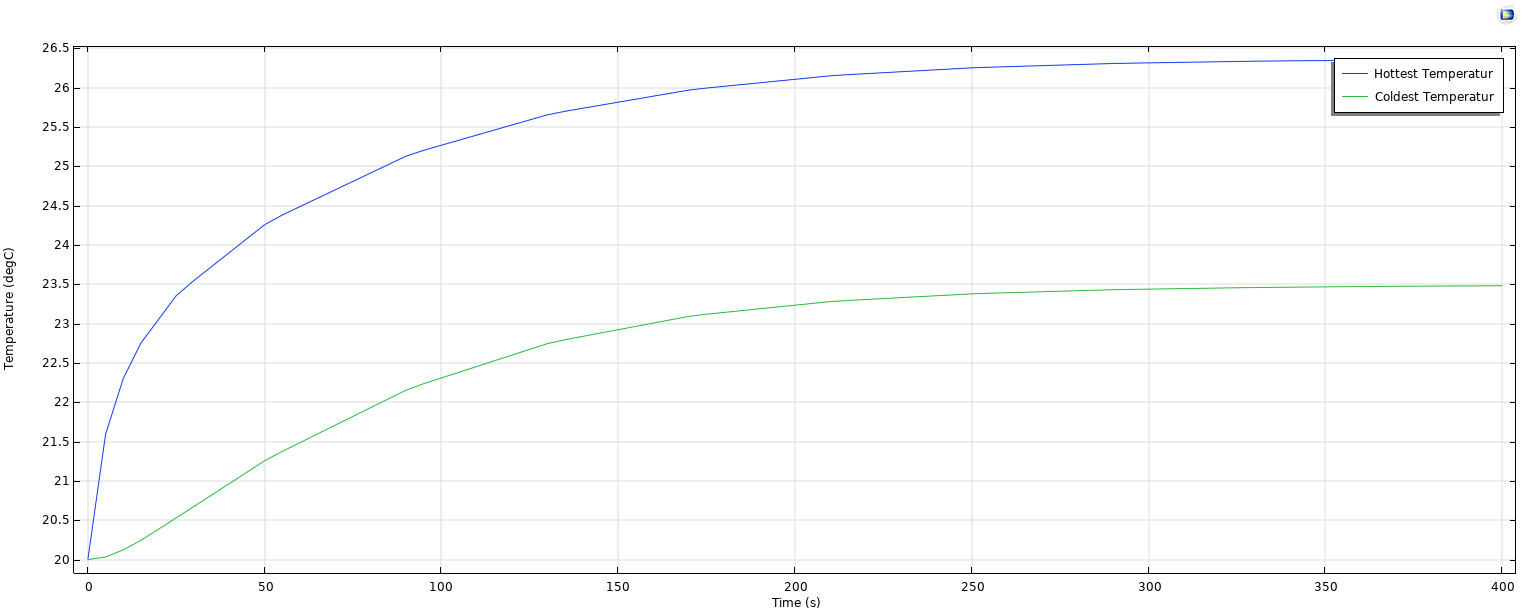
\includegraphics[width=\textwidth]{Bilder/time_dep.png}
	\captionof{figure}{Änderung der Temperatur mit der Zeit}
	\label{voltage}
\end{Figure}


Die Temperatur erhöht sich in der Simulation um $8,6 K$. 
Das unterschreitet die  händischen Berechnungen. Comsol verwendet andere Werte für die thermische Leitfähigkeiten.
Die Formeln, die man händischen löst sollen den Wert überschätzen, damit noch Sicherheit enthalten ist. 
Die händischen Formeln nehmen eine doppelt so große Fläche an auf der die Wärme abgegeben wird. 

Es wird der statische Endwert der Temperatur nach 700s erreicht. Danach ist die abgegebe Leistung = der eingeprägten Leistung

\noindent
\begin{thebibliography}{9}

\bibitem{Waermefluss}
Wuerth Elektronik eiSos  [online], [Zugriff am 22.12.2021] Verfuegbar unter:
 https://www.we-online.com/web/en/index.php/show/media/04
 \_leiterplatte/2011\_2/ relaunch/produkte\-5/heatsink/neu\_2011/
 TecReport\-01\-2011\-EN-S.pdf

% \bibitem{Vorlesung Aussteuerung}
% Prof. Dr. Reddig, Vorlesung Leistungselektronik

\bibitem{Elko}
TDK-Lambda Germany GmbH [online], [Zugriff am 22.12.2021] Verfuegbar unter:	https://www.emea.lambda.tdk.com/de/KB/Was-Sie-über-die-Lebensdauer-von-Stromversorgungen-wissen-sollten.pdf
Aachen, TDK-Lambda Germany GmbH



\bibitem{TI_Thermal}
Texas Instruments, 01.04.2013, Zugriff am 22.12.2021] Verfuegbar unter: https://www.ti.com/lit/pdf/snva419?keyMatch=
THERMAL\%20DESIGN\%20BY\%20INSIGHT\%20NOT\%
20HINDSIGHT

\bibitem{ipc}
IPC  [online], [Zugriff am 22.12.2021] Verfuegbar unter https://www.ipc.org/TOC/IPC-2221.pdf, United States, IPC

\bibitem{PCB_Querschnitt}
Cree, Inc. Optimizing PCB Thermal Performance for Cree XLamp LEDs 22.12.2010, [Zugriff am 22.12.2021] Verfuegbar unter https://www.digikey.de/en/articles/optimizing-pcb-thermal-performance-for-cree-xlamp-leds

\bibitem{aisler}
Aisler B. V.  [online], [Zugriff am 22.12.2021] Verfuegbar unter https://aisler.net/help/design-rules-and-specifications/specifications

% \bibitem{Vorlesung Aussteuerung}
% Prof. Dr. Reddig, Vorlesung Leistungselektronik



\end{thebibliography}

\end{multicols}
 

\end{document}
